\section{Julius}\label{Julius}
次にJuliusを\ruby{紹介}{しょう|かい}します。コマンド1つで試せるようにしてあります。下のようにターミナルにコマンドを打ちましょう。\\
\code{run-linux-gmm.sh}\\
このコマンドを打つと、いくらかシステム\ruby{情報}{じょう|ほう}が\ruby{表示}{ひょう|じ}された後、「<<please speak>>」という文字列が\ruby{現}{あらわ}れます( 図\ref{juliusの使い方})。

\begin{figure}[H]
\begin{center}
    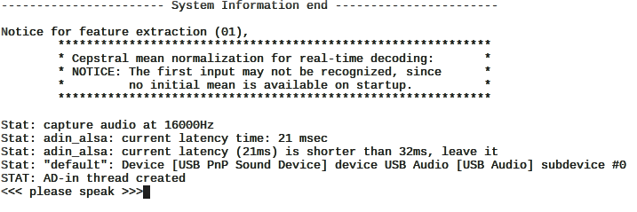
\includegraphics[width=\linewidth]{images/chap06/text06-img009.png}
    \caption{juliusの使い方}
    \label{juliusの使い方}
\end{center}
\end{figure}

その後マイクに向かって話しかければ、話しかけた単語が文字列になって画面に表示されます。今回は試しに果物の名前を話しかけてみましょう。
\begin{center}
	りんご みかん ぶどう もも あけび あんず いちご いちじく かき スイカ\\すもも 	なし メロン
\end{center}
	
終\ruby{了}{りょう}するときはCtrl+c(コントロールキーを\ruby{押}{お}しながらcを押す)を使います。<<please speak>>と表示されなくなり、pi@raspberrypi:と表示されればOKです。

Juliusはうまく言葉を\ruby{認識}{にん|しき}してくれましたか?おそらく、何度か間\ruby{違}{ちが}えて認識したと思います。日本語には数多の単語がありますし、\ruby{似}{に}た発音の単語もあるので、それらを完\ruby{璧}{ぺき}に認識することは\ruby{難}{むずか}しいのです。これを\ruby{解}{かい}決するために、「単語辞書」を登録してみましょう。\\

\begin{tcolorbox}[title=\useOmetoi]
\begin{enumerate}
        \addquiz{ターミナルにrun-linux-gmm.shと入力し、Juliusを試してみましょう。\\<<please speak>>と表示されたらマイクに向かって果物の名前を5つ話しかけましょう。\\何\ruby{個}{こ}認識されましたか?}
\end{enumerate}
\end{tcolorbox}
